\documentclass[11pt]{article}
\usepackage[margin=0.85in]{geometry}
\usepackage{graphicx} % Required for inserting images
\usepackage{natbib}
\usepackage{hyperref}
\usepackage{url}
\usepackage{amsmath}
\usepackage{booktabs}
\usepackage{subcaption}
\usepackage{caption}
\usepackage[most]{tcolorbox}
\usepackage[table]{xcolor}
\usepackage{float}

  \definecolor{claudebg}{RGB}{250,235,225}
  \definecolor{gptbg}{RGB}{225,235,250}
  \definecolor{owbg}{RGB}{235,240,230}

  \captionsetup{font=small,labelfont=bf}

  \title{Procedural Grep: Structural Variation for Agent Rollouts}
\author{Hamidah Oderinwale}
\date{May 2026}

\begin{document}

\maketitle

  \section{Abstract}

  Benchmark scores tell you what an agent got right; they do not tell you how it got there.
  \textcolor{blue}{We represent agent traces as structured objects in a shared procedure-space,
  so agents can be compared and audited by what they do rather than what they are named;
  procedural search---\emph{grep}---is one query interface over that representation, not the
  substance of it.} We apply this to evaluation datasets to study how structurally distinct
  tasks are (at a semantic and syntactic level), and
  how differently agents approach the same ones.  Among benchmarks, we find that procedural complexity across tasks is heavy-tailed. This matters as models saturate existing evals and
  questions arise about which are most valuable to develop
  further~\cite{kiela-etal-2021-dynabench}. We find that approaches are linked
  to model family, that structural similarity follows a long-tail distribution,
  and that structural representations carry signal not captured by natural
  language alone. We introduce \texttt{procgrep}, a library for auditing and evaluating agents for how they approach tasks at a procedural level given their traces in a top-down fashion.

\section{Introduction}
As programming becomes more high-level, program analysis needs to adapt beyond the syntax level to accommodate agents who can not only be optimized by the code they write but the actions they take. Improving agents will depend on procedural programmability and minimizing the gap between human intent and agent action. Additionally, it will involve assessing trajectories and holistic evaluations beyond binary outcomes \cite{haupt2025position}.

While chain-of-thought has proven itself (eliciting rationale from the agent) useful for post-hoc rationalizing---they cannot be taken as grounded accounts of action \cite{wei2023chainofthoughtpromptingelicitsreasoning,    ross2025modelingstudentlearning38, guan2025monitoringmonitorability}. Given this, in this work we explore representations from traces to turn them into structured objects and motivate the need for doing so, and we employ our suite of analytical tools to study the different trajectories that agents take outside controlled settings (in an area of work we call \emph{behavioral fingerprinting}). The goal is to expand the evaluation of agents beyond whether they simply pass or fail a task by venturing into the analysis of their procedural habits or ``style'' \cite{bisztray2025iknowllmwrote}. Additionally, we propose a number of interfaces and measurement frameworks to make these kinds of studies more accessible.

\section{Background}

As agent-style programming becomes more accessible, engineers will spend less time writing code directly and more time shaping how their agents frame and solve problems in the form of \emph{harnesses and scaffolds}---the wrappers around models that determine which tools they can employ, how they acquire context, and how they react to feedback. That said, traditional program analysis methods are too static to support this reliably and at scale \cite{jimenez2024swebenchlanguagemodelsresolve, yang2024sweagentagentcomputerinterfacesenable, chen2021evaluatinglargelanguagemodels, austin2021programsynthesislargelanguage}. In this work, we introduce a suite of procedural programming tools and analyses on agent traces from software engineering evaluations to address this problem. We motivate this work by showing how variation in agent behavior affects outcomes. While traces can be interpreted in isolation, there is much to gain from studying them in aggregate---tapping into collective wisdom \cite{surowiecki2004wisdom, Alizadeh_2015}---yet there is a lack of tools for doing so, as meaningful comparison calls for shared representations.

Previous work has explored solution variation at scale for MOOCs (massively online open courses) to observe behavior with clustering \cite{glassman2015overcode}. Platforms like LMArena compare agent outputs by evaluating prefered outputs in a pairwise fashion \cite{chiang2024chatbotarenaopenplatform}. Prior work has investigated using LLMs to generate plans from formal specifications~\cite{silver2024generalized}; with procedural representations it is possible to do the inverse, where queries can be written as procedural specs to `grep' traces.~\cite{yin2017syntacticneuralmodelgeneralpurpose}. Observational studies of LLM chats have been performed at scale to understand trends in model use \cite{tamkin2024clioprivacypreservinginsightsrealworld, deming2025how}. Frameworks have also been introduced for configuring models as agents to perform multi-step tasks with their own feedback loops given a goal specified upfront with `discovered' end states \cite{yao2023reactsynergizingreasoningacting}. And past work has also shown that coding style can be derived from source code using ASTs and decision trees in the form of random forest classifiers \cite{code_stylometry}. \textcolor{blue}{More recently, procedural fingerprinting has been applied at the pull-request level: coding agents leave distinguishable behavioral patterns across commit structure, PR format, and change concentration---enough that a classifier can identify which of five agents produced a PR at 97\% F1 from aggregate workflow features \cite{bisztray2025iknowllmwrote}. We extend this to the step-level trajectory, capturing the action sequence within a task attempt and revealing intra-trajectory structure---phase transitions, conditional decision logic, and training-lineage drift---that PR-level aggregates cannot observe.}

Existing frameworks have been built for code alone in siloed environments where context is missing, looking at patches \cite{GumTree2014, yin-neubig-2017-syntactic} with ASTs (abstract syntax trees) which generalizes across languages. We make use of established parsing methods and extend them to work in multi-modal free-form environments where prompts, for example, are written in natural language \cite{cruz2026textastherichestpreferencesignal} demonstrating that a rich set of features can be observed and made sense of. Next, given one's ability to audit procedures, there is an avenue for work which involves seeing what processes yield the best outputs. A new kind of model routing adapted to preferences could blossom from this direction. We explore it lightly in this work.

\section{A theory of procedural understanding}
Framing agent coding traces as procedures lets us comparatively study
and interact with them in ways that are useful for benchmarking,
evaluating the difficulty of evals themselves, differentiating models
by their behavioral fingerprints, and performing procedural search. We
release a library called ProcGrep to support these use cases. For
example, ProcGrep supports queries such as the following.

\begin{tcolorbox}[colback=black!3, colframe=black!30, boxrule=0.4pt,
  left=10pt, right=10pt, top=8pt, bottom=8pt, fontupper=\small]
All Claude-4 trajectories from the past two weeks on Python repositories
where \texttt{search\_repo} was followed by three or more
\texttt{read\_file} calls within the first 8 steps, the agent then made
at least one edit, and no \texttt{run\_test} occurred before the final
submit---on instances with difficulty score above 3.
\end{tcolorbox}

In this work, we use traces for a number of popular software engineering benchmarks and test a number of SOTA model families (GPT, Claude, DeepSeek, and Qwen). We use public archives of model traces for SWE-Bench (\url{princeton-nlp/SWE-bench-experiments}) and do the same for Agentless logs. We define what is the appropriate language to describe and program their behavior. What we call a ``procedural fingerprint'' is recovered from what an agent actually did (its trajectory) rather than its components or what it states. A fingerprint is a distinguishable feature of an agent from other agents and is consistent over time.

Firstly, we demonstrate that these fingerprints do in fact exist, and different models are differentiatable by their architectural types. First, we consider a distilled model pair, where there is a teacher and student model. \textcolor{blue}{While distilled models have been shown to achieve lower cost-per-task than their teacher models, it is not known whether the procedural habits that make teachers effective are also transferred---or whether distillation preserves outcomes while altering the underlying decision structure. We find that the child inherits the parent's full action vocabulary but shows concentrated entropy ($+$0.23 bits), outcome-dependent drift (passing trajectories are 12pp more parent-like than failing ones at native resolution), and conditional divergence at every thinking step---suggesting that output-only supervised fine-tuning transfers surface behavior but not the diagnostic loop that enables course-correction.}

Given a set of procedures that we might want to compare, which we can call a procedural space, we need a vocabulary or a set of actions or subroutines that we can use to describe all of them. The contributions of this framework comes from being able to define this vocabulary bottom-up instead of with a more hard-coded or classifier based approach. We benchmark our methods against prompt-based classifiers, finding that \textcolor{blue}{across four judge models, prompt-based classifiers label 17--38\% of instances as compositionally divergent with near-zero cross-family agreement ($\kappa < 0.05$), demonstrating that natural-language descriptions of procedural divergence are unstable}. This affirms our motivations for having representations that can be shared across models and instances to allow for comparative analysis.

Across all models, passing behavior includes a higher ratio of browsing to other actions. Extended thinking Claude models spend the largest proportion of their time in the shell compared to older models with more even task breakdowns. Models in the GPT family have more consistent behavior, but newer ones spend more time editing.  Agent harnesses have less task diversity, potentially due to their programmed behavior and have more distinct breakdowns, the Agentless scaffold spends a disproportionate amount of time browsing and the Moatless scaffold leads to a large proportion of testing. An interesting application of this is forecasting the costs of an agent, as it is not only a product of the cost per tool call, but a function of the operation types needed to complete it and the procedural tendencies of the model being orchestrated.

\begin{figure}[h]
    \centering
    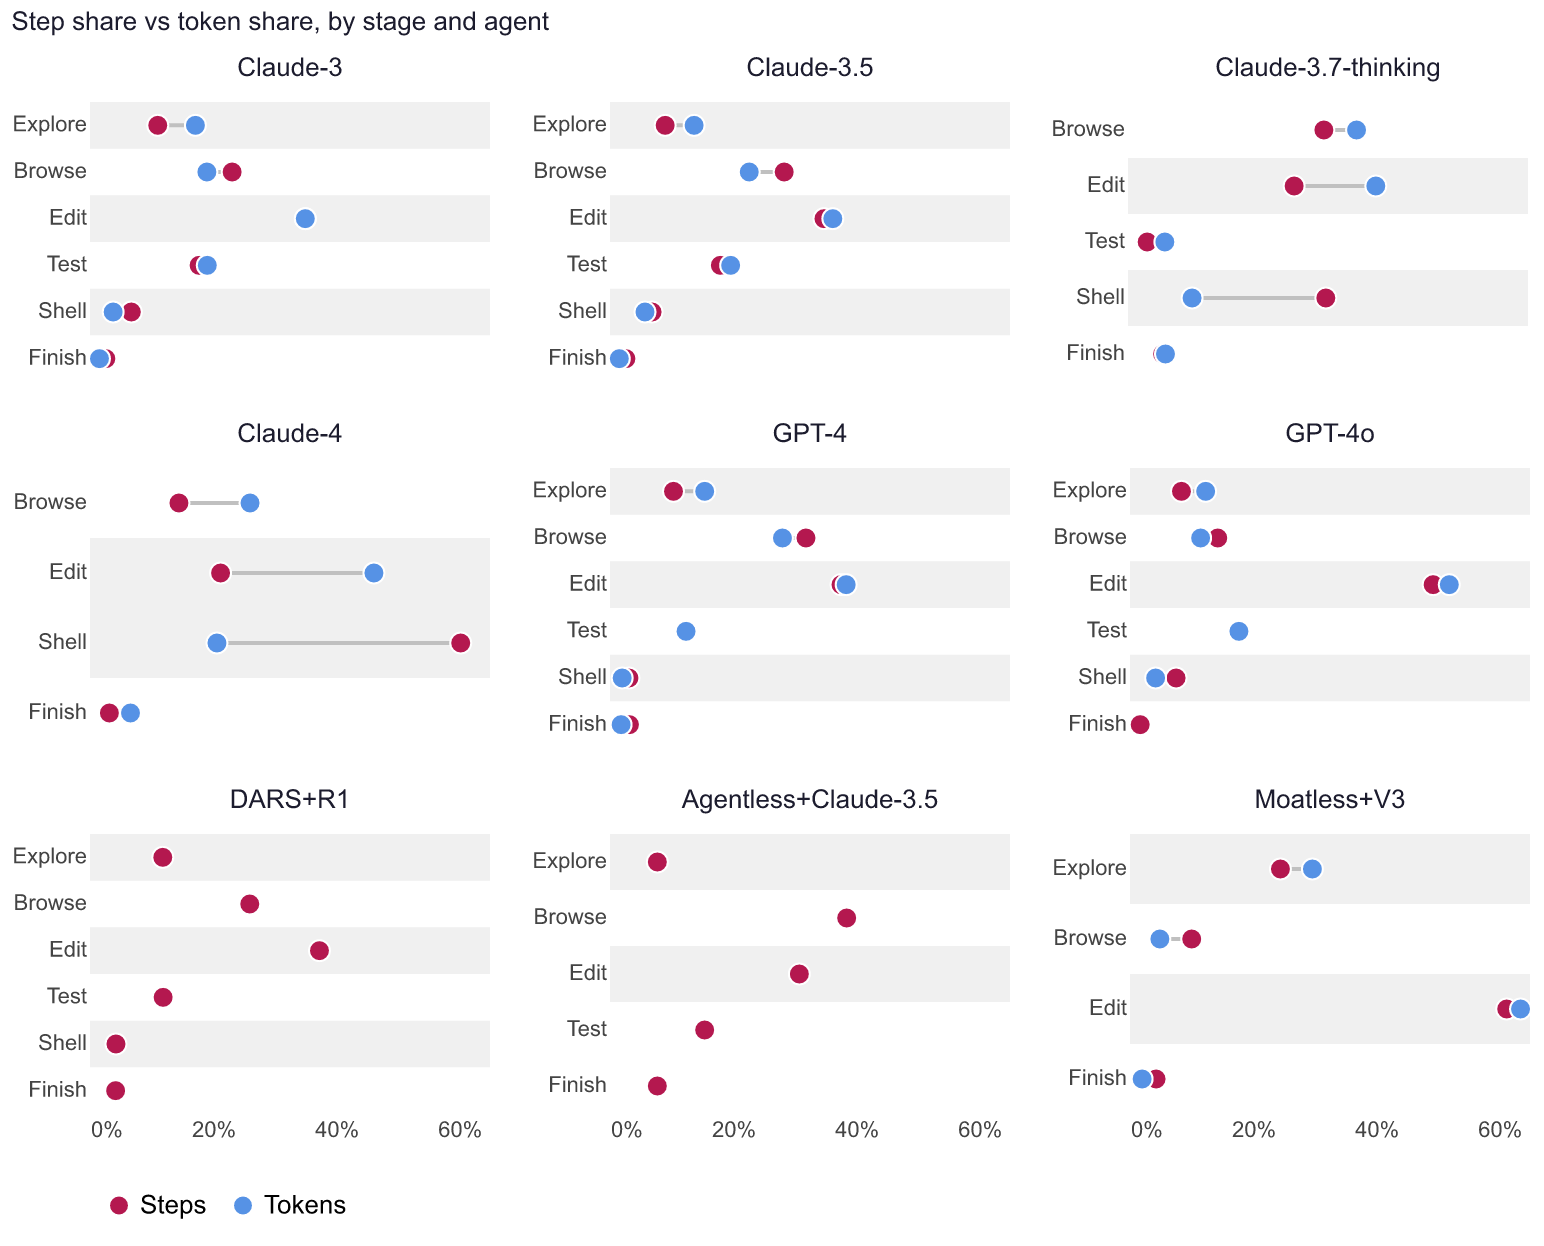
\includegraphics[width=0.6\linewidth]{figures/fig_step_vs_token_cost.png}
    \caption{Cost breakdown of agents by operation type and tokens.}
    \label{fig:step_token_cost}
\end{figure}

\begin{figure}[h]
    \centering
    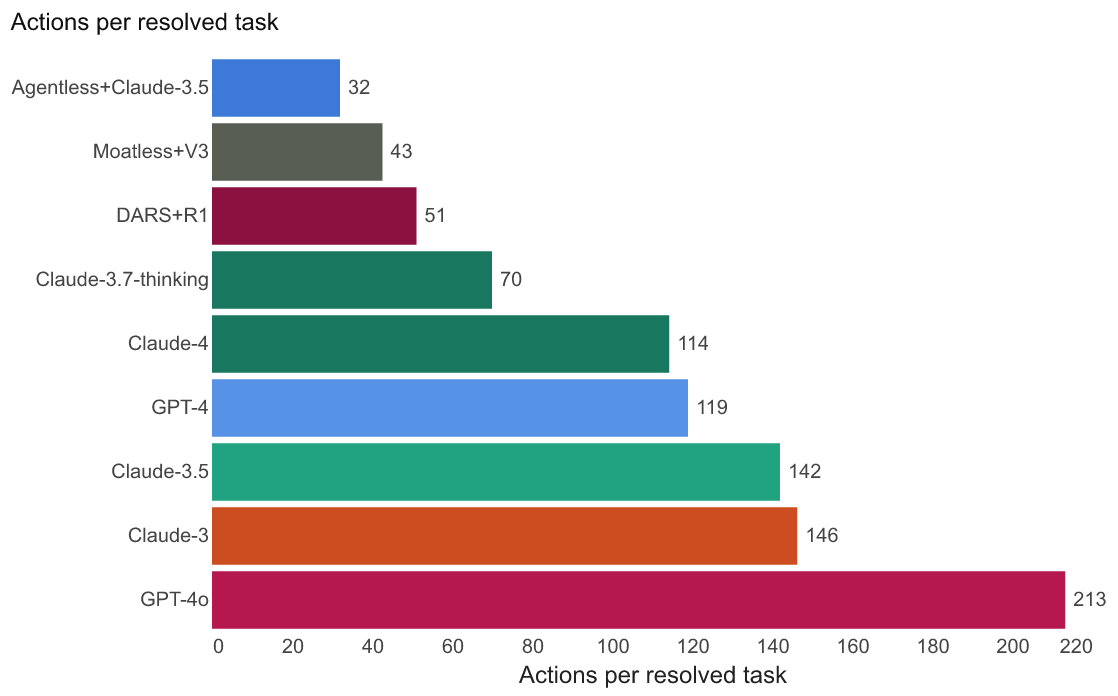
\includegraphics[width=0.4\linewidth]{figures/fig_steps_per_resolved.png}
    \caption{Average number of steps per resolved tasks across agents.}
    \label{fig:steps_resolved}
\end{figure}

  \begin{table*}[H]
  \centering\footnotesize\setlength{\tabcolsep}{4pt}
  \resizebox{\linewidth}{!}{%
  \begin{tabular}{lllrrrrrrrrr}
  \toprule
  \textbf{Scaffold} & \textbf{Model} & \textbf{Paradigm}
    & \textbf{$n$} & \textbf{Resolve} & \textbf{Steps}
    & \textbf{Repertoire} & \textbf{Compr.} & \textbf{Entropy}
    & \textbf{Cost/task} & \textbf{\$/step} & \textbf{Cost/resolved} \\
   & & & & & \textbf{/traj} & \textbf{@90\%} & \textbf{ratio}
    & \textbf{(bits)} & & & \\
  \midrule
  \rowcolor{claudebg}
  SWE-agent & Claude-3 Opus        & RLHF dense        & 300 & 11.7\% & 17.1 & 44 & 0.537
  & 5.58 & \$3.42 & \$0.200 & \$29.31 \\
  \rowcolor{claudebg}
  SWE-agent & Claude-3.5           & RLHF dense        & 289 & 23.9\% & 32.7 & 42 & 0.559
  & 5.56 & \$1.62 & \$0.050 & \textcolor{blue}{\$7.06}  \\
  \rowcolor{claudebg}
  SWE-agent & Claude-3.7-thinking  & Extended thinking & 284 & 50.7\% & 33.6 & 32 & 0.471
  & 5.14 & \$0.78 & \$0.023 & \$1.53  \\
  \rowcolor{claudebg}
  SWE-agent & Claude-4             & Extended thinking & 288 & 59.0\% & \textbf{64.8} & 35
   & 0.417 & 5.26 & \$1.19 & \$0.018 & \$2.02  \\
  \midrule
  \rowcolor{gptbg}
  SWE-agent & GPT-4                & RLHF dense        & 300 & 18.0\% & 21.4 & 40 & 0.443
  & 5.47 & \$2.51 & \$0.117 & \$13.93 \\
  \rowcolor{gptbg}
  SWE-agent & GPT-4o               & RLHF dense        & 278 & 19.8\% & 39.1 & \textbf{49}
   & 0.425 & 5.76 & \$2.53 & \$0.065 & \textcolor{blue}{\$13.82} \\
  \midrule
  \rowcolor{owbg}
  DARS      & DeepSeek-R1          & RL reasoning      & 300 & 47.0\% & 24.0 & 19 &
  \textbf{0.572} & 4.44 & \$2.43$^*$ & --- & \$5.17$^*$ \\
  \rowcolor{owbg}
  Agentless & Claude-3.5           & RLHF dense        & 300 & 40.7\% & 13.0 & \textbf{1}
  & \textbf{0.077} & \textbf{0.00} & \$0.50$^*$ & --- & \$1.23$^*$ \\
  \rowcolor{owbg}
  Moatless  & DeepSeek-V3          & MoE pretrain      & 300 & 30.7\% & 13.1 & 12 & 0.417
  & 3.71 & \$0.02 & ${\approx}0$ & \$0.06 \\
  \bottomrule
  \end{tabular}%
  }
  \\[0.3em]
  {\footnotesize $^*$Cost estimated. \$/step = cost per inference call.
Extended thinking models reduce cost per step by routing calls through the shell
and orchestrating them before invoking the more expensive inference calls
(Claude-4: \$0.018/step vs.\ Claude-3: \$0.200/step).}
  \caption{Per-agent procedural fingerprint and cost efficiency on SWE-bench Verified
  ($n=2{,}639$).}
  \label{tab:per-agent-megatable}
  \end{table*}

 \begin{table}[h]
  \centering\small
  \begin{tabular}{lccc}
  \toprule
  \textbf{Representation} & \textbf{n} & \textbf{F1 (k=1)} & \textbf{Source} \\
  \midrule
  Structural pattern overlap  & 289 & 0.347 & Deterministic \\
  Action sequence distance    & 289 & 0.274 & Deterministic \\
  Edit operation overlap      & 289 & 0.256 & Deterministic \\
  Narrative description       & 289 & 0.177 & Varies by model \\
  Agent plan description      & 289 & 0.155 & Varies by model \\
  Divergence classifier (LLM) & 87--286 & 0.000--0.363 & $\kappa < 0.05$ (cross-family) \\
  \midrule
  Random retrieval            & 289 & 0.13--0.24 & Baseline \\
  \bottomrule
  \end{tabular}
  \caption{Pass/fail prediction F1 at $k{=}1$ nearest neighbours and cross-model
    stability across representations. The divergence classifier was run across four
    judge models (GPT-4o, GPT-4o mini, Llama~3.3~70B, Qwen~2.5~72B); A range of F1 scores
  are aggregated across model types. Random retrieval baseline reflects the pass rate
  under class imbalance (12--24\% positive); structural representations achieve a genuine
  lift of $+$0.10--0.22 above this floor.}
  \label{tab:representation_comparison}
  \end{table}

\textcolor{blue}{A prompt-based classifier (GPT-4o as judge) labels 38\% of instance pairs as compositionally divergent, with agreement dropping to near zero across model families ($\kappa < 0.05$); see Table~\ref{tab:divergence_by_model} in the Appendix. This instability motivates the structural vocabulary below.} This means that there are features of the full vocabulary or alphabet which we can study in itself and can form the basis of insights. To define our vocabulary, we need to be able to extract these subroutines and label them to understand what they are. Each subroutine should be composable and collapse into one another because steps are taken in sequence for specific tasks and to avoid redundancy---where each subroutine of a procedure should be meaningfully unique or composed of unique sub-subroutines.

\textcolor{purple}{TODO: Add vocabulary size baseline from Table 1 (Repertoire@90\% column) and describe what this says about procedural diversity across agents.}

BPE or Byte-Pair Encoding is a useful analog for this process. While BPE chunks natural language tokens by merging those that frequently appear together to compress the data for pre-training LLMs, we chunk operations from generated code \cite{sennrich2016neuralmachinetranslationrare}. \textcolor{blue}{The idea of learning a compact vocabulary bottom-up from procedural traces connects to program synthesis work on library learning~\cite{ellis2020dreamcodergrowinggeneralizableinterpretable}, where recurring program fragments are abstracted into reusable subroutines; here the corpus drives vocabulary induction rather than a task-specific objective.} Like BPE, our vocabulary is learned or derived from the procedures themselves rather than hand-specified, and when a subroutine is added to the vocabulary it is now a meaningful member of an alphabet. With BPE, however, there is no dynamic stopping point for the algorithm which means that a target vocabulary size needs to be set up front.

\begin{figure}[h]
    \centering
    \includegraphics[width=0.78\linewidth]{figures/trace_pipeline.png}
    \caption{Illustrative figure of the process of vocabulary induction given an agent trace.}
    \label{fig:encoding_pipeline}
\end{figure}

We consider the induction of a vocabulary to be a similar class of problem to a clustering one, so we draw on how clustering algorithms are evaluated to form the basis of an emergent stopping criterion \cite{rosenberg-hirschberg-2007-v}. We use the V-measure as our evaluation for the mined patterns. We consider a vocabulary stable when it maximizes two measures: completeness, meaning the subunits of each chunk are correctly aligned with an intent, and homogeneity, meaning a chunk contains only operations that belong to it. \textcolor{blue}{We call a vocabulary \emph{optimal} when it best balances two competing pressures: \emph{expressiveness}---enough granularity to capture genuine variation in how agents approach a task \cite{glassman2015overcode}---and \emph{canonicalization}---collapsing surface-level naming differences so procedures with the same intent compare as the same. These are the two quantities V-measure trades off: homogeneity rewards expressiveness (a chunk holds only operations that belong together, so distinct approaches stay distinct), while completeness rewards canonicalization (an intent's operations group into one chunk rather than scattering). The optimum is the harmonic-mean balance, not either extreme.} \textcolor{blue}{See Figure~\ref{fig:vmeasure} in the Appendix; the canonical alphabet stabilises across V\,=\,64--128 and the native alphabet peaks at V\,=\,256.}

\[
V = 2 \cdot \frac{h \cdot c}{h + c}
\]

where homogeneity $h$ and completeness $c$ are defined as

\[
h = 1 - \frac{H(\text{ops} \mid \text{subroutine})}{H(\text{ops})} \qquad c = 1 - \frac{H(\text{subroutine} \mid \text{ops})}{H(\text{subroutine})}
\]

$H(\text{ops} \mid \text{subroutine})$ measures the confidence of belonging of an operation to a chunk, and $H(\text{subroutine} \mid \text{ops})$ measures the reverse. A vocabulary is stable when $V$ is maximized.

To extract the operations themselves, we take code hunks---solution patches---from these evaluation datasets and then parse them with an AST that gives a node tree and a syntactical and semantic representation of the code. Given the structural representation of the solution patches, we then apply an embedding stage to encode the change in plain language and the underlying intent by contextualizing the structured patch with the surrounding code and a behavioral description from the model.

\textcolor{blue}{Another property of the optimal vocabulary is that the procedures it contains are distinguishable and non-redundant. While BPE merges by frequency, an alternative is to mine contiguous sequential patterns directly. We compare both methods: at equivalent pattern count ($K=64$), BPE achieves V-measure 0.253 versus 0.213 for frequency-ranked contiguous $n$-grams, and continues improving to 0.290 at $V=128$ while $n$-gram clustering plateaus. BPE's hierarchical merging builds discriminative multi-step procedures more efficiently than a flat frequency list.}

We investigate entropy within the context of a collective with Jensen-Shannon Divergence. Entropy (H), a measure of uncertainty in a distribution (where a distribution here is the probability over all the possible actions in our vocabulary), is a property that can be applied to a single agent's distribution of actions, where it is defined as: $$H(a) = -\sum_{v \in \mathcal{V}} p_a(v) \log_2 p_a(v)$$ JSD allows us to build on entropy and measure how different two distributions are and is defined as: $$\mathrm{JSD}(a, b) = H\!\left(\frac{p_a + p_b}{2}\right) - \frac{1}{2}H(a) -
  \frac{1}{2}H(b)$$ This is a useful foundation when weighing options for developer decision-making and model routing. Given pairwise orderings, it is then possible to come up with partial orderings which is useful for ranking results with methods like Bradley-Terry.

  \section{Why procedural representations matter}

Given theoretical grounding, we put foundations to work in a number of ways. In this section we look at top-down analyses given agent traces.  Firstly, we show that these approaches offer a more grounded representation of process than what can be elicited from models in natural language alone. We ask two questions: given what a model says it will do, what does it actually do (forward faithfulness)? Then, given what a model says it did, what did it actually do (reverse faithfulness)? We find that both model families have complete reverse faithfulness, where every action they take is mentioned somewhere in their reasoning.

\begin{figure}[h]
    \centering
    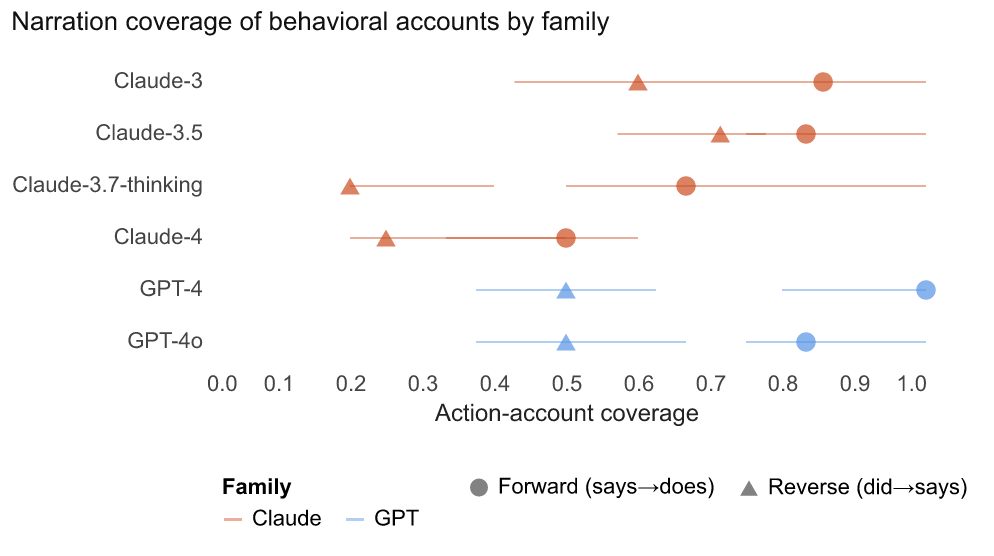
\includegraphics[width=0.42\linewidth]{figures/cot_alignment_6agents.png}
    \caption{Faithfulness to behavioral accounts for Claude and GPT model families.}
    \label{fig:cot_alignment}
\end{figure}

Then, we consider precision in the behavioral descriptions themselves. We find that models are generally verbose in their accounts, which might be a signal of performative chain-of-thought \cite{boppana2026reasoningtheaterdisentanglingmodel}. For example, the GPT family are trained with heavy RLHF and instruction-tuning. Whereas the Claude family of models are presumably trained to follow more sprawling reasoning patterns before coalescing them into some preferred approach.  Extended thinking models are the most verbose and have similar behavior to the baseline of shuffled rationales.

   \begin{table}[h]
  \centering
  \small
  \begin{tabular}{lrrrrr}
  \toprule
  \textbf{Model} & \textbf{n} & \textbf{Verbosity} & \textbf{Precision} &
  \textbf{Baseline} & \textbf{Recall} \\
  \midrule
  \rowcolor{claudebg} Claude-3            & 300 & 1.07 & 0.833 & 0.678 & 0.857 \\
  \rowcolor{claudebg} Claude-3.5          & 289 & 1.00 & 0.857 & 0.732 & 0.833 \\
  \rowcolor{claudebg} Claude-3.7-thinking & 284 & 1.35 & 0.625 & 0.623 & 0.800 \\
  \rowcolor{claudebg} Claude-4            & 288 & 1.32 & 0.500 & 0.536 & 0.750 \\
  \midrule
  \rowcolor{gptbg}    GPT-4               & 300 & 1.17 & 0.800 & 0.713 & 1.000 \\
  \rowcolor{gptbg}    GPT-4o              & 278 & 1.18 & 0.750 & 0.679 & 1.000 \\
  \midrule
   \rowcolor{owbg} DARS+R1 & 300 & 1.07 & 0.857 & 0.775 & 0.875 \\
  \bottomrule
  \end{tabular}
  \end{table}

\section{Natural experiments with procedural representations}

With this data, we can also validate other kinds of inferences regarding the shapes of problems and model behavior. For example, past work has found that models struggle with compositional generalization---this means that they are brittle in contexts where they need to do incremental work. We validate this in the wild and find that problems that require compositional generalization, defined by problems that have nested subroutines, are especially difficult for agents, as evidenced by their failure rates. We define compositional problems as ones where the subproblems are ones that have been solved by the agent before, but when put together the agent failed. Looking at Figure~\ref{fig:compositional_failure} we can observe that compositionality is a relatively strong signal of failure, followed by novel primitives, and familiar patterns yield the lowest failure rates. However, the pattern holds the most strongly for RLHF-trained models and much more modest for more classically trained models. Across models, similar trends hold, but open-weight agents have lower failure rates to compositional problems---When computing the difference of open-weight model failure at all points compared to other model families is ${\sim}9\%$.

Additionally, we look at different agent pipelines and compare them across 289 tasks (Agentless v. SWE-Bench Agent). Agentless successfully solves 63 more tasks than SWE-Agent and we can use the procedural methods for assessing why.

  \begin{table}[t]
  \centering\small
  \begin{tabular}{lrrrr}
  \toprule
  \textbf{Outcome} & \textbf{$n$} & \textbf{Difficulty}
    & \textbf{SWE-agent steps} & \textbf{Agentless steps} \\
  \midrule
  Both pass       &  54 & 7.17 & 20.4 & 13.0 \\
  SWE-agent only  &  15 & 4.53 & 30.7 & 13.0 \\
  Agentless only  &  63 & 4.59 & 33.3 & 13.0 \\
  Neither passes  & 157 & 0.69 & 36.8 & 13.0 \\
  \midrule
  \multicolumn{2}{l}{Total} & & 289 \\
  \bottomrule
  \end{tabular}
  \caption{Outcomes of two agent scaffolds on 289 tasks.}
\label{tab:scaffold_outcomes}
  \end{table}

\begin{figure}[h]
      \centering
      \begin{subfigure}[t]{0.28\linewidth}
          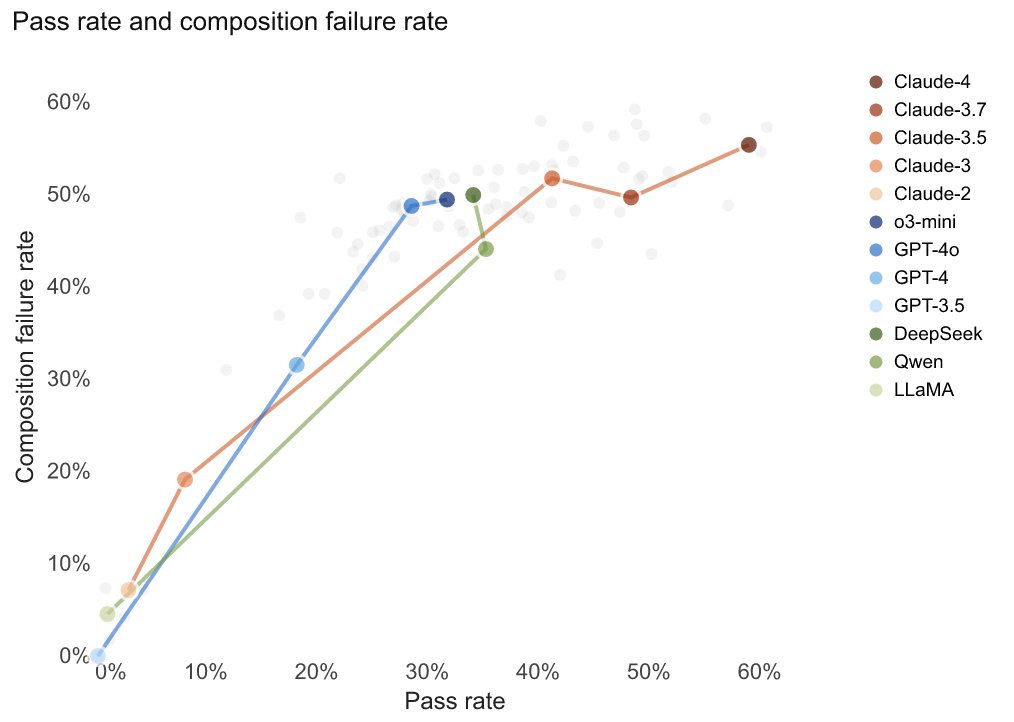
\includegraphics[width=\linewidth]{figures/failure_mix_by_agent_84.png}
          \caption{Relationship between compositional problems and pass rate across
  models.}
          \label{fig:compositional_failure}
      \end{subfigure}
      \hfill
      \begin{subfigure}[t]{0.56\linewidth}
          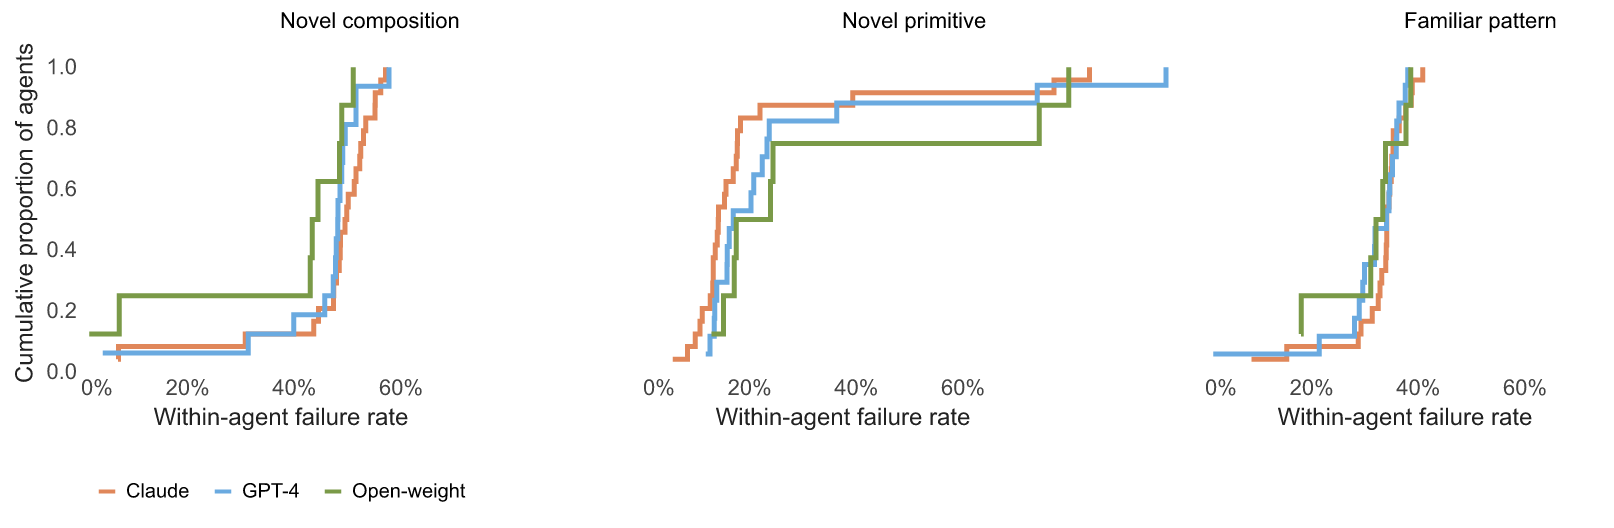
\includegraphics[width=\linewidth]{figures/failure_by_family.png}
          \caption{Failure type distributions by model family.}
          \label{fig:failure_by_family}
      \end{subfigure}
      \caption{Model behavior on compositional tasks.}
      \label{fig:composition_analysis}
  \end{figure}

Next, developers make a number of decisions to train and scaffold their models. We set out to understand how this affects model processes based on a set of tasks and find that ``fingerprints'' are recoverable---unique model-specific patterns regarding tool-use and order of operations. Given certain parameters like the costs for different types of operations and the length of a task, this can form the basis of more informed model choice and configuration decisions depending on a developer's goal (i.e.\ task and workflow-aware routing). For a given model, its procedural space can be described by its entropy and compression, where entropy describes the variance of the actions and compression is a rough proxy for repetitiveness. We find the GPT-4o has the most diversity of actions compared to Claude models.

\textcolor{blue}{Fingerprints also surface exploration style. Claude-3.5 opens the most files per trace (mean 2.41 vs.\ 1.66--1.90 for peers) and degrades the least when spreading across multiple files: pass rate drops from 29.0\% (1 file) to 17.6\% (3+ files), compared to GPT-4o's 27.3\%~$\to$~8.1\%. Claude-3.5 spreads wider and degrades less for doing so.}

  \textcolor{purple}{TODO: Add multi-file exploration findings here as proper prose --- GPT-4: 23.5\%→7.7\% at 3+ files, Claude-3.5 least degradation (29.0\%→17.6\%), mean 2.41 files opened vs 1.66-1.90 for peers. Source: rich\_features analysis.}

  \subsection{In-task monitoring}

\textcolor{blue}{The structural patterns \texttt{procgrep} validates retrospectively are detectable early enough to be operational. Consider the \texttt{stuck\_reading} pattern (\texttt{read\_file}$\to$\texttt{think}$\to$\texttt{read\_file}$\to$\texttt{think}), which fires on 21 of 23 parent-pass/child-fail matched instances. In 80\% of those cases the pattern completes by step~12---before the trajectory has consumed most of its context budget. A trajectory that reaches step~12 in a read loop will typically run to exhaustion (150+ steps in the longest failures) without ever reaching the implementation phase, spending ${\sim}835$ tokens per 5-step read cycle versus ${\sim}210$ tokens for Claude-4's productive test-driven loop---a 4$\times$ cost ratio on a trajectory already heading toward failure. Detecting this at step~6 (median) and re-prompting recovers the context budget before it is exhausted.}

\textcolor{blue}{This makes pattern-based monitoring a resource management tool, not just an evaluation artifact. The following shows a minimal inference setup that exposes the per-step token counts needed for real-time detection:}

\begin{tcolorbox}[colback=black!3, colframe=black!30, boxrule=0.4pt,
  left=10pt, right=10pt, top=8pt, bottom=8pt, fontupper=\small]
\textcolor{blue}{
\texttt{python -m sglang.launch\_server}~\textbackslash\\
\texttt{~~--model-path SWE-bench/SWE-agent-LM-32B}~\textbackslash\\
\texttt{~~--tp 1}~\textbackslash\\
\texttt{~~--enable-metrics}~\textbackslash\\
\texttt{~~--enable-cache-report}~\textbackslash\\
\texttt{~~--cuda-graph-max-bs 8}
}
\end{tcolorbox}

\textcolor{blue}{With \texttt{--enable-cache-report} active, each turn returns \texttt{usage.completion\_tokens} and \texttt{cache\_hit\_tokens}. Matched against the \texttt{stuck\_reading} spec entry, this gives a circuit-breaker trigger: if the contiguous pattern completes within the first 12 steps, interrupt and re-prompt. Tensor parallelism and quantization are model-dependent; these two flags are the minimum for per-step procgrep capture at any serving scale.}

\section{Controlled evaluations with procedural controls}

In agent programming and benchmarking, an engineer can specify parameters such as the number of tool use turns and response lengths in the form of tokens, but there is little control over how a task is done. Controlling for behavior at the level of actions and operations is an under-explored way of assessing capabilities---while ablations are possible at different levels of abstraction, it is not possible to say a model can only retrieve context via grep or when, or run a certain number of tests and after what operations.

Fingerprints give us behavioral trends that form the basis for predicting
which actions a given agent is most likely to take, useful for next-action
prediction and anomaly detection. We batch trajectories into five groups, training models on four and
leaving one as a held-out control. As shown in Table~\ref{tab:trajectory_holdouts},
agents fall into three regimes: deterministic scaffolds like Agentless,
which are nearly fully predictable (82\% accuracy, $+$51 points over baseline);
constrained scaffolds like Moatless, where the scaffold drives behavior
and the baseline is already high (73\% accuracy, $+$8 points); and
open-ended model-driven agents like Claude and GPT, where predictions
are stronger at the single-action level (e.g., Claude-3.5 at 50\%
accuracy, $+$33 points). This makes the case for procedural representations
as a basis for prediction. We also find that edit streaks are a strong
failure signal: for Moatless+DeepSeek-V3, 43\% of trajectories have edit
streaks of 5 or more, and of those, the fail rate is 80\%, compared to
59\% for no-streak trajectories. For Claude-3.5 the signal is weaker,
with pass rate dropping from 26\% to 11\% with a streak $\geq$5, though
the magnitude is comparable.

\textcolor{blue}{Trajectory length is itself a strong, model-agnostic failure signal (Figure~\ref{fig:regression_length}): pass rate declines monotonically from 70\% at 1--10 steps to 9\% beyond 60 steps. Because length accrues observably as a trajectory runs, this is directly actionable as an early-stopping or escalation trigger.}

\begin{figure}[h]
    \centering
    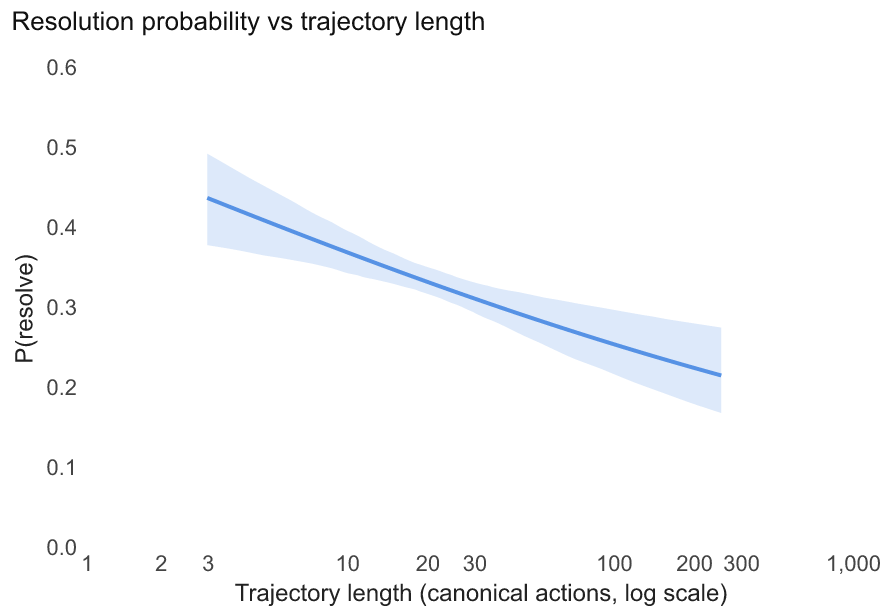
\includegraphics[width=0.58\linewidth]{figures/fig_regression_length.png}
    \caption{Pass rate by trajectory length. Longer trajectories are strongly associated with failure, declining from 70\% (1--10 steps) to 9\% ($>$60 steps).}
    \label{fig:regression_length}
\end{figure}

\begin{table}[htbp!]
\centering\small\setlength{\tabcolsep}{4pt}
  \begin{tabular}{lrrrrrr}
  \toprule
  & \multicolumn{3}{c}{\textbf{Next action}}
  & \multicolumn{3}{c}{\textbf{Next stage}} \\
  \cmidrule(lr){2-4}\cmidrule(lr){5-7}
  \textbf{Agent} & Base & Acc. & $\Delta$ & Base & Acc. & $\Delta$ \\
  \midrule
  \rowcolor{claudebg}
  Claude-3              & 13\% & 46\% & $+$33 & 33\% & 47\% & $+$14 \\
  \rowcolor{claudebg}
  Claude-3.5            & 18\% & 50\% & $+$33 & 35\% & 51\% & $+$16 \\
  \rowcolor{claudebg}
  Claude-3.7-thinking   & 23\% & 54\% & $+$31 & 44\% & 65\% & $+$21 \\
  \rowcolor{claudebg}
  Claude-4              & 51\% & 61\% & $+$10 & 51\% & 67\% & $+$16 \\
  \midrule
  \rowcolor{gptbg}
  GPT-4                 & 20\% & 57\% & $+$37 & 50\% & 56\% & $+$6  \\
  \rowcolor{gptbg}
  GPT-4o                & 27\% & 60\% & $+$34 & 50\% & 62\% & $+$12 \\
  \midrule
  \rowcolor{owbg}
  DARS+DeepSeek-R1      & 30\% & 46\% & $+$17 & 37\% & 49\% & $+$12 \\
  \rowcolor{owbg}
  Agentless+Claude-3.5  & 31\% & 82\% & $+$51 & 31\% & 82\% & $+$51 \\
  \rowcolor{owbg}
  Moatless+DeepSeek-V3  & 65\% & 73\% & \textbf{$+$8}
                        & 65\% & 73\% & \textbf{$+$8} \\
  \bottomrule
  \end{tabular}
  \caption{Next-action and next-stage prediction accuracy across agent trajectories.}
  \label{tab:trajectory_holdouts}
  \end{table}

\textcolor{blue}{Beyond prediction, procedural specifications open a path to \emph{programming} and rewarding agent behavior on long-horizon tasks: a YAML reward spec assigns partial credit over procedural milestones (phases, penalties, bonuses) rather than a single binary pass/fail. We treat this as an illustrative capability of the system rather than a validated training result---the full reinforcement-learning loop is not demonstrated here---and detail the spec, a worked scoring example, and its application to the distilled model in Appendix~\ref{app:reward}. Closing that loop is left to future work.}

\section{\textcolor{blue}{Case Study: SFT Distillation}}
\label{sec:distillation}

\textcolor{blue}{SWE-agent-LM-32B is produced by the SWE-smith pipeline \cite{yang2025swesmith}: Claude-3.7~Sonnet (the teacher) generates trajectories on SWE-bench tasks, passing trajectories are filtered and used as supervised demonstrations, and Qwen2.5-32B is fine-tuned on the result. Supervision is on \emph{outputs only}---the student learns to reproduce the teacher's actions but not the reasoning behind them. We analyse 284 parent and 498 child trajectories using \texttt{lineage\_diff} across four axes: vocabulary preservation, entropy shift, outcome-stratified overlap, and conditional structure drift.

At the canonical level, the child uses every atom type the parent uses (Jaccard~$=~1.0$). Despite identical coverage, the per-trajectory entropy has shifted: parent mean 2.31 bits, child 1.99 bits ($-$0.23 bits). The child's procedure distributions are more concentrated---SFT filtered for the parent's passing trajectories, and the child over-learned that focus into rigidity.

Stratifying by outcome at the native level: passing child trajectories share 0.64 of the parent's tool signatures; failing trajectories share only 0.52 ($\Delta = 0.12$). The mean conditional JSD is 0.043 (canonical), with the largest impact at \texttt{think}: JSD~$=~0.052$ across 8,453 parent occurrences. After every thinking step, the child chooses a different next action from what the parent would choose. The surface habit transferred; the decision logic did not.}

\begin{figure}[h]
  \centering
  \begin{subfigure}[t]{0.32\linewidth}
    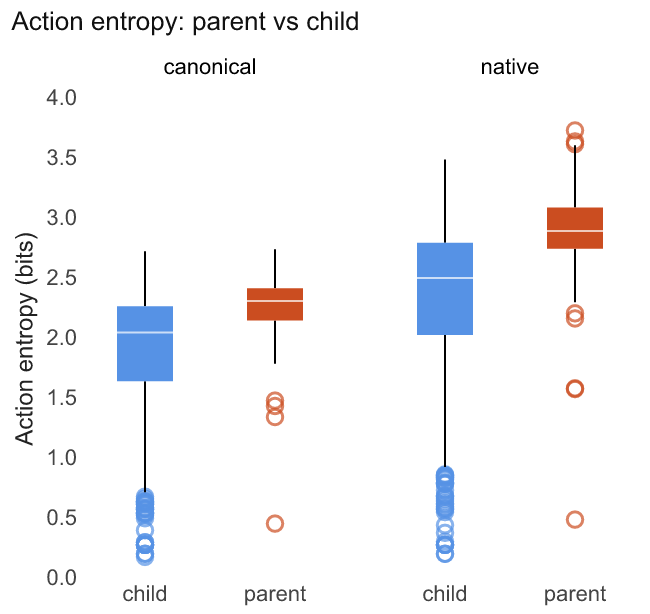
\includegraphics[width=\linewidth]{figures/fig_distillation_A_entropy.png}
    \caption{\textcolor{blue}{Action entropy: parent vs.\ child at canonical and native levels. The child distribution is more concentrated ($-$0.23 bits).}}
    \label{fig:dist_entropy}
  \end{subfigure}\hfill
  \begin{subfigure}[t]{0.38\linewidth}
    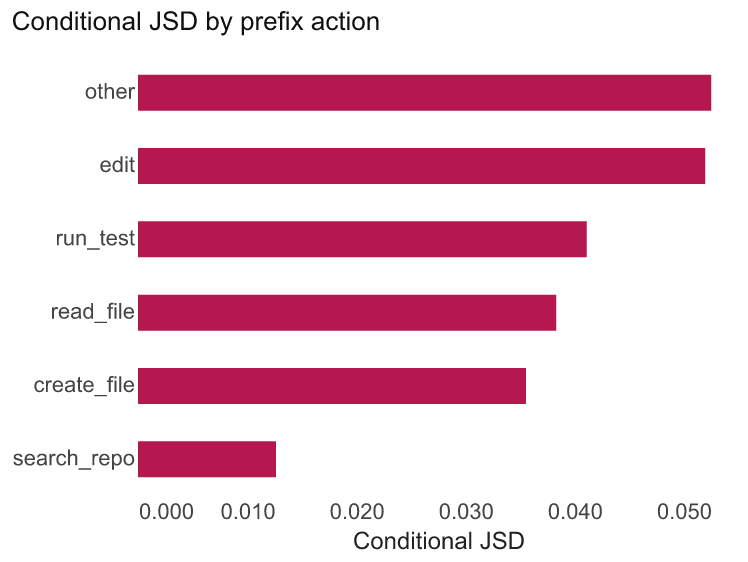
\includegraphics[width=\linewidth]{figures/fig_distillation_B_conditional.png}
    \caption{\textcolor{blue}{Conditional JSD by prefix action type, ranked by frequency-weighted impact. \texttt{think} leads at 8,453 parent occurrences.}}
    \label{fig:dist_conditional}
  \end{subfigure}\hfill
  \begin{subfigure}[t]{0.26\linewidth}
    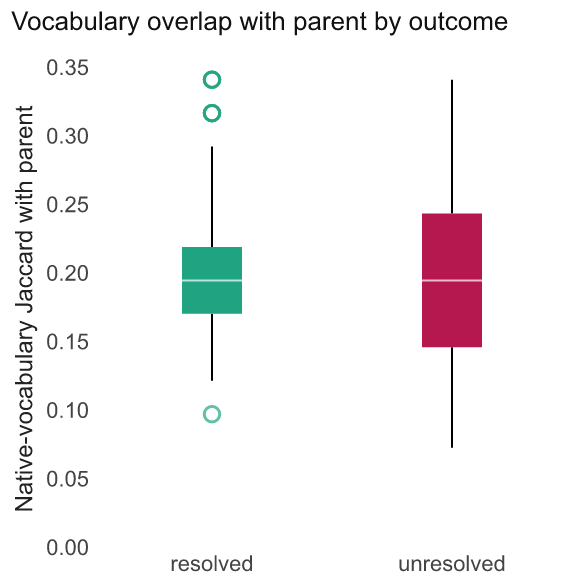
\includegraphics[width=\linewidth]{figures/fig_distillation_C_outcome.png}
    \caption{\textcolor{blue}{Native vocabulary Jaccard with parent by outcome. Canonical~$=~1.00$ both strata (stated in text).}}
    \label{fig:dist_outcome}
  \end{subfigure}
  \caption{\textcolor{blue}{Distillation case study: Claude-3.7~Sonnet (parent) $\to$ SWE-agent-LM-32B (child). Vocabulary is fully preserved at canonical level but the distribution concentrates, failing trajectories diverge further from the parent than passing ones, and decision logic drifts at every thinking step.}}
  \label{fig:distillation}
\end{figure}

\textcolor{purple}{TODO: Add entropy null result --- the -0.23 bit shift is directed (child always lower than parent); across unrelated agent pairs entropy shifts are larger and undirected. This validates that the concentration is specific to the distillation relationship.}

\section{Future work}

\textcolor{blue}{Prior work on behavioral diffing and model-diffing has compared model outputs at the response level. Three directions follow from this work. First, \emph{lineage attribution at scale}: applying \texttt{lineage\_diff} across pairs of open-weight models on HuggingFace to ask whether procedural fingerprints can identify training relationships when the relationship is not disclosed. Second, \emph{procedural regression detection} across model releases---the Claude-3.7$\to$Claude-4 opening-move shift (JSD\,=\,0.27 at step~1) shows that training-recipe changes surface as procedural discontinuities. Third, correlating procedural axes with model attributes through observational regression; this can generate hypotheses for controlled distillation experiments like the one in \S\ref{sec:distillation}.}

\section{Appendix}

\subsection{\textcolor{blue}{Procedural reward modeling (illustrative)}}
\label{app:reward}

\textcolor{blue}{Typically reward systems for coding models have focused on binary states, but trajectory specifications enable partial rewards based on procedural milestones. We present the specification and scoring as an illustration of the system; we do not train against it here. A reward spec (YAML) defines phases, penalties, and bonuses over the canonical atom sequence:}

\begin{tcolorbox}[colback=black!3, colframe=black!30, boxrule=0.4pt,
  left=10pt, right=10pt, top=8pt, bottom=8pt, fontupper=\small]
\textcolor{blue}{
\texttt{phases:}\\
\texttt{~~- name: exploration~~~~reward: 0.10}\\
\texttt{~~~~require\_any: [\{atom: search\_repo\}, \{atom: read\_file\}]}\\
\texttt{~~~~min\_occurrences: 2~~~~before\_first: edit}\\
\texttt{~~- name: test\_verification~~~~reward: 0.25}\\
\texttt{~~~~require\_sequence: [edit, run\_test]~~~~max\_gap: 5}\\
\texttt{~~- name: iterative\_refinement~~~~reward: 0.20}\\
\texttt{~~~~require\_sequence: [run\_test, think, edit]}\\
\texttt{penalties:}\\
\texttt{~~- name: edit\_streak~~~~penalty: 0.15}\\
\texttt{~~~~pattern: [edit, edit, edit, edit, edit]~~~~contiguous: true}\\
\texttt{~~- name: stuck\_reading~~~~penalty: 0.10}\\
\texttt{~~~~pattern: [read\_file, think, read\_file, think]~~~~contiguous: true}\\
\texttt{bonuses:}\\
\texttt{~~- name: test\_driven~~~~reward: 0.10}\\
\texttt{~~~~require\_sequence: [run\_test]~~~~before\_first: edit}
}
\end{tcolorbox}

\textcolor{blue}{Scoring a trajectory against this spec returns a structured reward record:}

\begin{tcolorbox}[colback=black!3, colframe=black!30, boxrule=0.4pt,
  left=10pt, right=10pt, top=8pt, bottom=8pt, fontupper=\small]
\textcolor{blue}{
\texttt{\{"instance\_id": "django\_\_django-12345",}\\
\texttt{~~"binary\_pass": false,~~~~"proc\_score": 0.55,}\\
\texttt{~~"satisfied\_phases": ["exploration", "diagnosis",}\\
\texttt{~~~~~~~~~~~~~~~~~"implementation", "test\_verification"],}\\
\texttt{~~"triggered\_penalties": ["edit\_streak"],}\\
\texttt{~~"triggered\_bonuses": []\}}
}
\end{tcolorbox}

\textcolor{blue}{Scoring the distilled child model yields mean procedural score 0.795 across 498 trajectories---with passing trajectories scoring 0.902 versus 0.723 for failing ones ($\Delta = 0.179$). Notably, 87.8\% of child trajectories trigger the \texttt{stuck\_reading} penalty, compared to 87.7\% of the teacher---confirming this failure mode was inherited, not introduced by fine-tuning. The teacher achieves mean procedural score 0.940 with a tighter pass/fail gap (0.953 vs.\ 0.927). The full reward spec and scorer are available at \texttt{from procgrep.reward import load\_spec, score}. Whether optimizing against this score improves performance is left to future work.}

\begin{figure}[h]
    \centering
    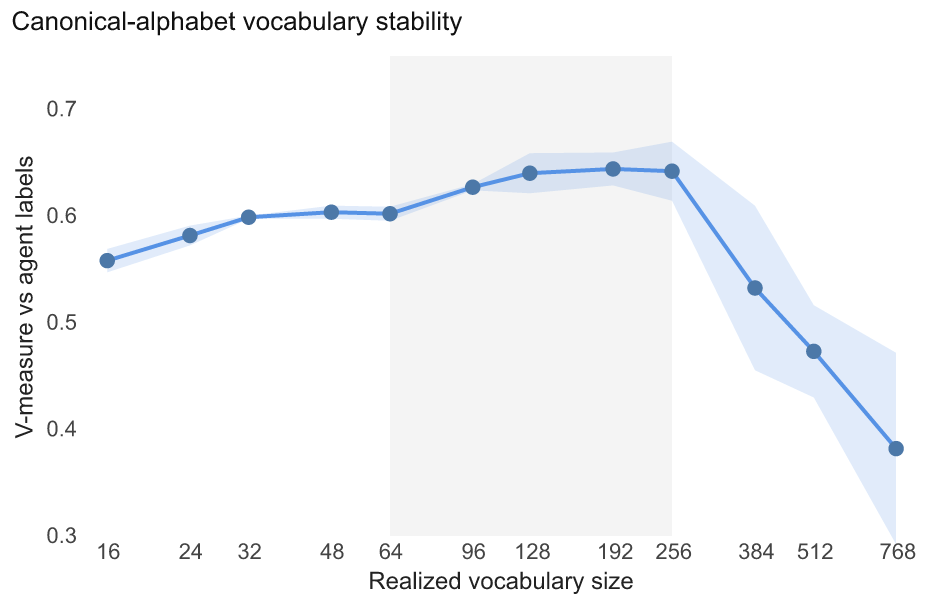
\includegraphics[width=0.6\linewidth]{figures/fig_vmeasure_sweep.png}
    \caption{\textcolor{blue}{V-measure of BPE vocabulary clustering against agent labels as a function of vocabulary size. The canonical alphabet stabilises across V\,=\,64--128 (peak at V\,=\,128, V-measure\,=\,0.290); the native alphabet peaks at V\,=\,256 (V-measure\,=\,0.410). These values justify the vocabulary sizes used throughout this work.}}
    \label{fig:vmeasure}
\end{figure}

\begin{figure}[h]
    \centering
    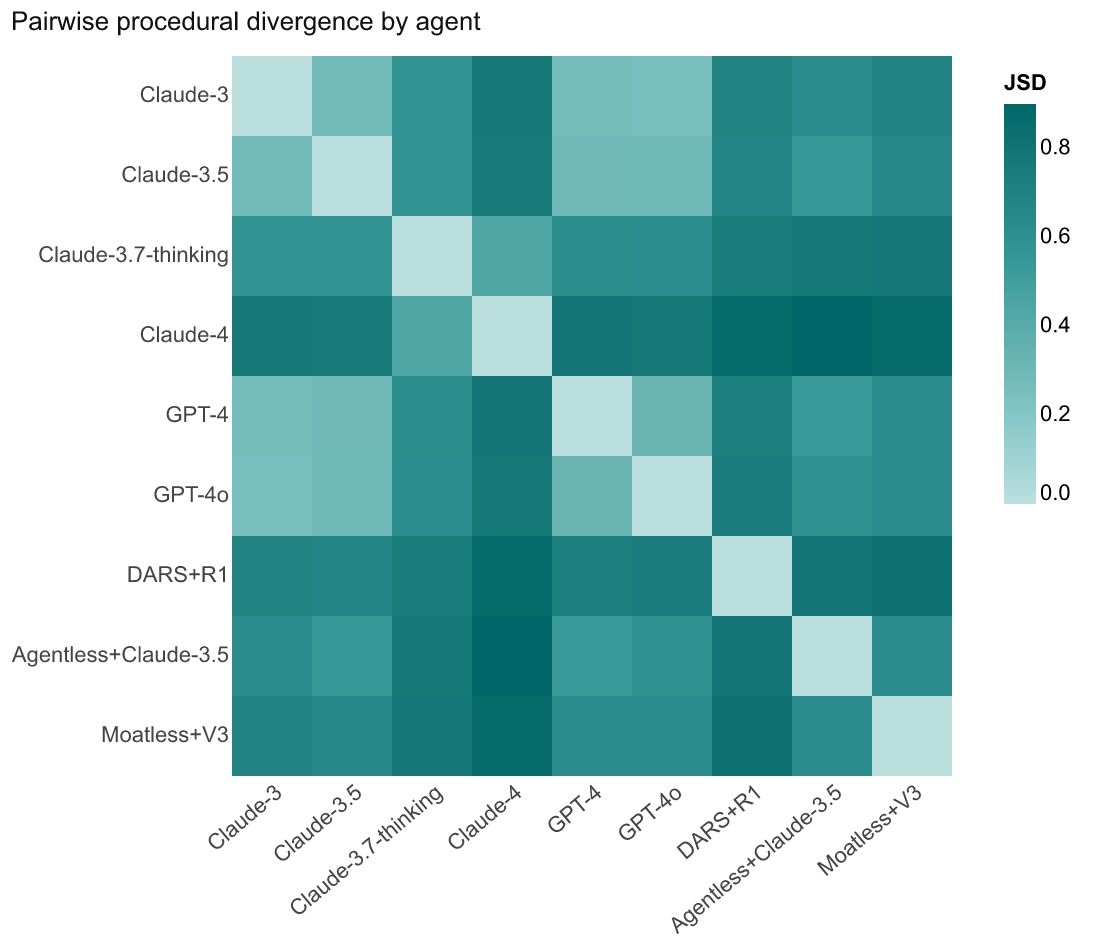
\includegraphics[width=0.66\linewidth]{figures/fig_jsd_matrix_full_canonical.png}
    \caption{\textcolor{blue}{Pairwise JSD between 10 agents at canonical alphabet, grouped by model family and scaffold. The distilled child (SWE-agent-LM-32B) is closest to its parent (Claude-3.7~Sonnet) at JSD\,=\,0.10. The same model under two harnesses (Claude-3.7 SWE-agent vs.\ tools format) diverges at JSD\,=\,0.49, confirming scaffold\,$>$\,era\,$>$\,lineage in procedural impact.}}
    \label{fig:jsd_full}
\end{figure}

  \begin{table}[h]
  \centering\small
  \begin{tabular}{lcccc}
  \toprule
  \textbf{Judge model} & \textbf{n} & \textbf{F1 (k=1)} & \textbf{\% compositional} &
  \textbf{Mean $\kappa$} \\
  \midrule
  GPT-4o         & 286 & 0.363 & 38.1\% & 0.124 \\
  GPT-4o mini    & 285 & 0.246 & 36.5\% & 0.144 \\
  Qwen 2.5 72B   &  87 & 0.167 & 17.2\% & 0.128 \\
  Llama 3.3 70B  &  87 & 0.000 & 21.8\% & 0.123 \\
  \midrule
  Weighted mean  & 745 & 0.253 & -- & -- \\
  \bottomrule
  \end{tabular}
  \caption{Classification results per judge model and divergence. Near-zero inter-model agreement ($\kappa < 0.05$) motivates the structural vocabulary approach.}
  \label{tab:divergence_by_model}
  \end{table}

\begin{figure}[h]
    \centering
    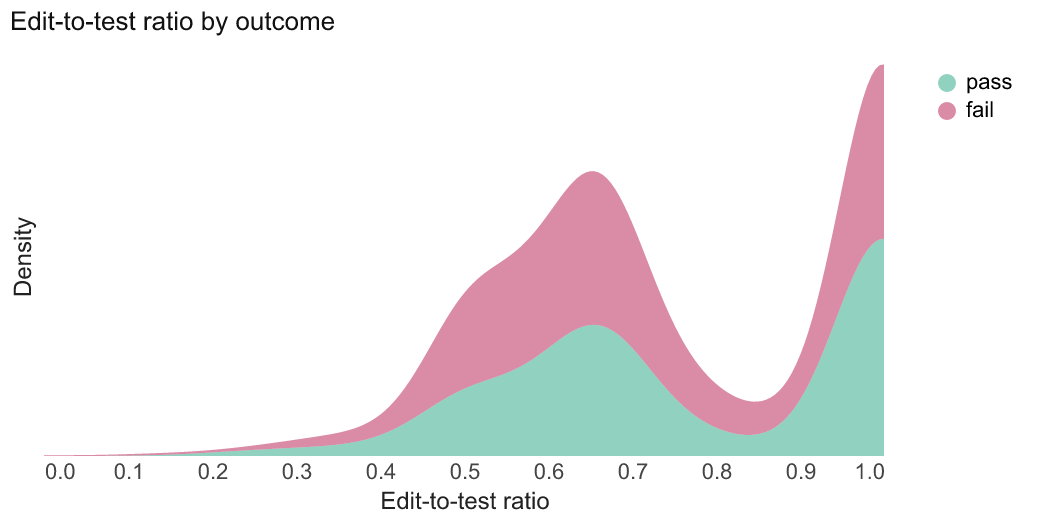
\includegraphics[width=0.58\linewidth]{figures/fig_regression_edit_test.png}
    \caption{\textcolor{blue}{Edit-to-test ratio distribution by outcome. Passing trajectories peak near ratio\,=\,0.5; failing trajectories have a long tail at high edit-to-test ratios, consistent with the edit-streak failure signal.}}
    \label{fig:regression_edit_test}
\end{figure}

\begin{figure}[h]
    \centering
    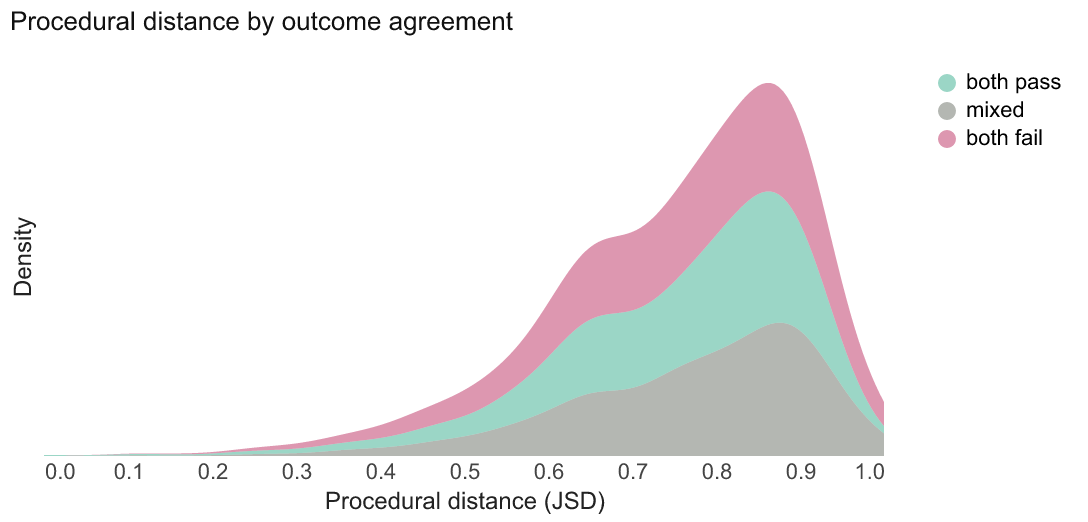
\includegraphics[width=0.64\linewidth]{figures/fig12_tier1b_sodp.png}
    \caption{\textcolor{blue}{Procedural distance by outcome agreement on matched instances. Both-pass pairs (green) cluster at low JSD; both-fail pairs (red) spread to higher procedural distance.}}
    \label{fig:sodp}
\end{figure}

\begin{figure}[h]
    \centering
    \includegraphics[width=0.64\linewidth]{figures/fig13_discriminative_bigrams.png}
    \caption{\textcolor{blue}{Discriminative action transitions between agent pairs. Claude-4 overuses \texttt{create\_file}$\to$\texttt{run\_test}; the child overuses \texttt{think}$\to$\texttt{read\_file}, reflecting its read-heavy exploration style.}}
    \label{fig:bigrams}
\end{figure}

\textcolor{purple}{TODO: Add harness decomposition result as a paragraph or table --- scaffold (JSD 0.49) > model era (JSD 0.36) > training lineage (JSD 0.15). This is the controlled ablation that validates the canonical/native alphabet hierarchy.}

\bibliography{main}
\bibliographystyle{apalike}
\end{document}
